\documentclass[10pt]{beamer}
\usefonttheme{professionalfonts,serif}
\def\newblock{\hskip .11em plus .33em minus .07em}
\usepackage[numbers,sort]{natbib}
\renewcommand{\rmdefault}{psbx}
\usepackage[utf8]{inputenc}
\usepackage[T1]{fontenc}
\usepackage{textcomp}
\usepackage{eulervm}

\usetheme{default}           % tips from David Blei
\useinnertheme{circles}
\useoutertheme{infolines}
\setbeamertemplate{headline}{}
\setbeamertemplate{navigation symbols}{}
\setbeamerfont{itemize/enumerate subbody}{size=\normalsize}
\setbeamerfont{itemize/enumerate subsubbody}{size=\normalsize}
\usecolortheme{seahorse}
\setbeamersize{text margin left=2mm,text margin right=2mm}

\graphicspath{{../../figures/}}

\definecolor{mypine}{rgb}{0.05,0.45,0.05}
\definecolor{mycyan}{rgb}{0.0,0.9,0.9}
\newcommand{\Red}{\textcolor{red}}
\newcommand{\Blue}{\textcolor{blue}}
\newcommand{\Green}{\textcolor{mypine}}
\newcommand{\PineGreen}{\textcolor{mypine}}
\newcommand{\Magenta}{\textcolor{magenta}}
\newcommand{\Cyan}{\textcolor{mycyan}}

\newcommand{\N}{\mathcal{N}}
\newcommand{\R}{\mathbb{R}}
\newcommand{\T}{{\scriptsize^{\top}}}
\newcommand{\D}{\mathcal{D}}
\newcommand{\F}{\mathcal{F}}
\newcommand{\E}{\mathbb{E}}
\newcommand{\V}{\mathbb{V}}
\newcommand{\M}{\mathcal{M}}
\newcommand{\KL}{\mathcal{KL}}
\newcommand{\cut}[1]{}
\newcommand{\trace}{\operatorname{trace}}

\newcommand{\bmu}{{\boldsymbol{\mu}}}
\newcommand{\btheta}{\boldsymbol{\theta}}
\newcommand{\bepsilon}{\boldsymbol{\epsilon}}
\newcommand{\balpha}{\boldsymbol{\alpha}}
\newcommand{\bbeta}{\boldsymbol{\beta}}
\newcommand{\bphi}{\boldsymbol{\phi}}
\newcommand{\bPhi}{\boldsymbol{\Phi}}
\newcommand{\bSigma}{\boldsymbol{\Sigma}}
\newcommand{\bpi}{\boldsymbol{\pi}}
\newcommand{\blambda}{\boldsymbol{\lambda}}

\newcommand{\argmax}{\operatorname{argmax}}
\newcommand{\argmin}{\operatorname{argmin}}
\newcommand{\ci}{{\bot\negthickspace\negthickspace\bot}} % conditional indep.
\newcommand{\neigh}{\operatorname{ne}}
\newcommand{\vectr}[2]{  \left[ \!\!\begin{array}{c} #1 \\
      #2 \end{array} \!\!\right]}
\newcommand{\deff}{\stackrel{\mathrm{def}}{=}}
\newcommand{\deldel}[2]{\frac{\partial #1}{\partial #2}}

\newcommand{\maketilde}{\raisebox{0.4ex}{\tiny $\sim$}}
\newcommand{\bfa}{\mathbf a}
\newcommand{\bfb}{\mathbf b}
\newcommand{\bfe}{\mathbf e}
\newcommand{\bff}{\mathbf f}
\newcommand{\bfk}{\mathbf k}
\newcommand{\bfm}{\mathbf m}
\newcommand{\bfn}{\mathbf n}
\newcommand{\bfp}{\mathbf{p}}
\newcommand{\bfs}{\mathbf s}
\newcommand{\bfu}{\mathbf u}
\newcommand{\bfx}{\mathbf x}
\newcommand{\bfy}{\mathbf y}
\newcommand{\bft}{\mathbf t}
\newcommand{\bfv}{\mathbf v}
\newcommand{\bfw}{\mathbf w}
\newcommand{\bfA}{\mathbf A}
\newcommand{\bfI}{\mathbf I}
\newcommand{\bfK}{\mathbf K}


\title{Gaussian process covariance functions}
\author{Carl Edward Rasmussen}
\date{October 20th, 2016}

\begin{document}

\begin{frame}
\titlepage
\end{frame}

\begin{frame}
\frametitle{Key concepts}

\begin{itemize}
\item chose covariance functions and use the marginal likelihood to
\begin{itemize}
\item set hyperparameters
\item chose between different covariance functions
\end{itemize}
\item covariance functions and hyperparameters can help
  \Blue{interpret} the data
\item we illutrate a number of different covariance function families
\begin{itemize}
\item stationary covariance functions: squared exponential, rational
  quadratic and Mat\'ern forms
\end{itemize}
\item many existing models are special cases of Gaussian processes
\begin{itemize}
\item radial basis function networks (RBF)
\item splines
\item large neural networks
\end{itemize}
\item combining existing simple covariance functions into more
  interesting ones
\end{itemize}

\end{frame}

\begin{frame}
\frametitle{Model Selection, Hyperparameters, and ARD}

We need to determine both the \emph{form} and \emph{parameters} of
the covariance function. 
We typically use a \Blue{hierarchical model}, where the parameters of
the covariance are called \Blue{hyperparameters}. 

A very useful
idea  is to use \Blue{automatic relevance determination (ARD)} covariance
functions for feature/variable selection, e.g.:
\[
k({\bf x},{\bf x}') = v_0^2\exp\big(\!-\sum_{d=1}^D\frac{(x_d-x_d')^2}{2v_d^2}
\big),\text{\ \ \ \ \ \ hyperparameters\ }
\theta=(v_0,v_1,\ldots,v_d,\sigma^2_n).
\]
\centerline{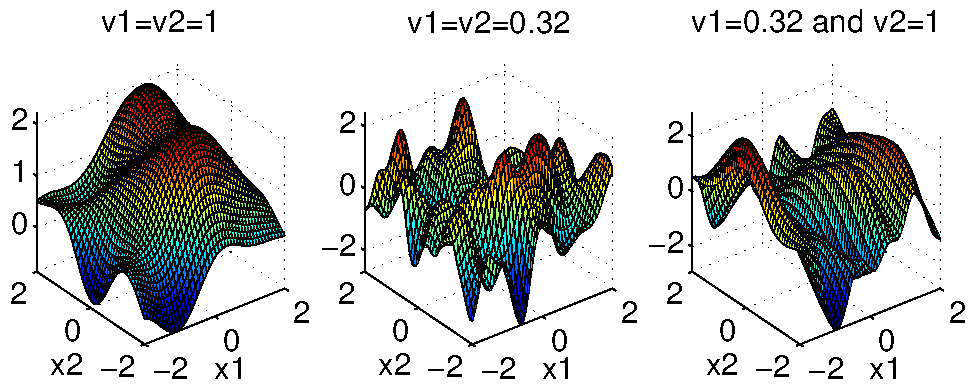
\includegraphics[width=0.9\textwidth]{ardprior}}
\end{frame}

\begin{frame}
\frametitle{Rational quadratic covariance function}

The \emph{rational quadratic} (RQ) covariance function, where $r=x-x'$:
%
\[
k_{\rm RQ}(r)\;=\;\Big(1+\frac{r^2}{2\alpha\ell^2}\Big)^{-\alpha}
\label{e:covRQ}
\]
%
with $\alpha, \; \ell > 0$ can be seen as a \emph{scale mixture} (an infinite
sum) of squared exponential (SE) covariance functions with different
characteristic length-scales.

Using $\tau=\ell^{-2}$ and
$p(\tau|\alpha,\beta)\propto\tau^{\alpha-1}\exp(-\alpha\tau/\beta)$:
\[
\begin{split}
k_{\rm RQ}(r)\;=\;&\int p(\tau|\alpha,\beta)k_{\rm SE}(r|\tau)d\tau\\
\propto\;&\int\tau^{\alpha-1}\exp\Big(\!-\frac{\alpha\tau}{\beta}\Big)
\exp\Big(\!-\frac{\tau r^2}{2}\Big)d\tau\;\propto\;
\Big(1+\frac{r^2}{2 \alpha \ell^2}\Big)^{-\alpha},
\end{split}
\label{e:rq}
\]
\end{frame}

\begin{frame}
\frametitle{Rational quadratic covariance function II}

\begin{center}
\begin{tabular}{cc}
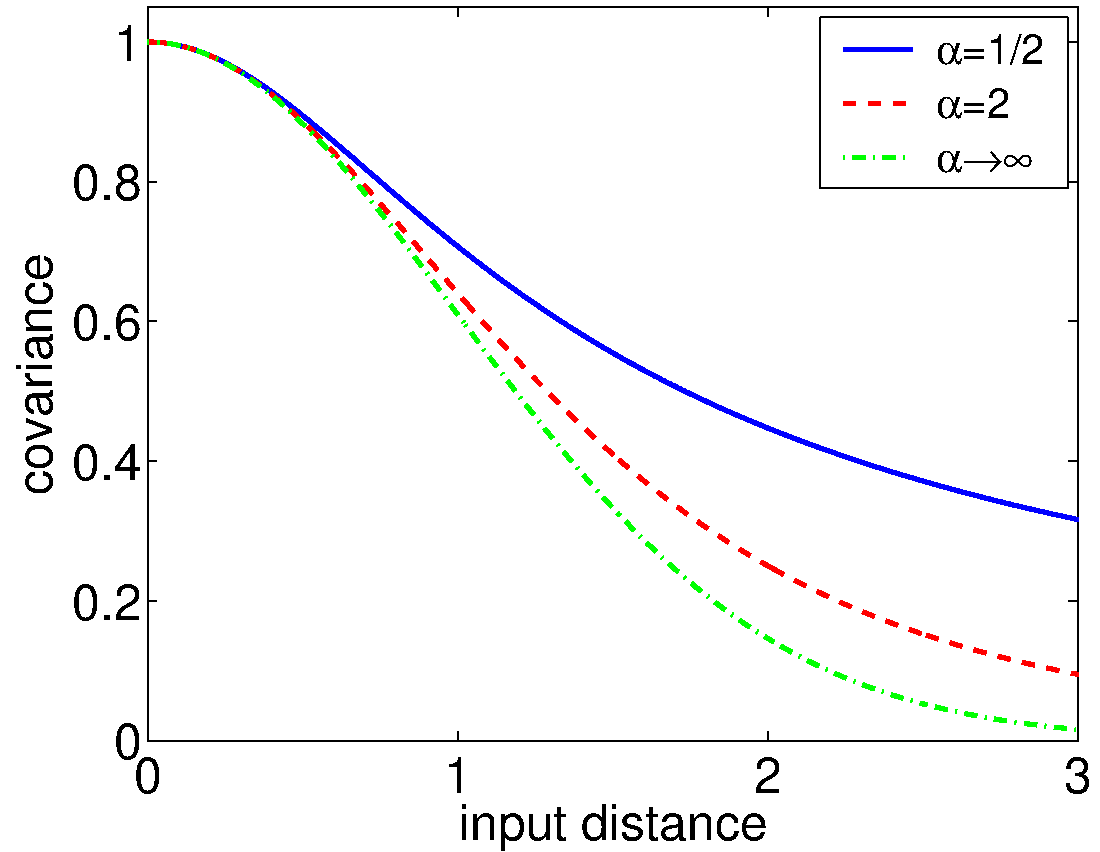
\includegraphics[width=0.45\textwidth]{rq} &
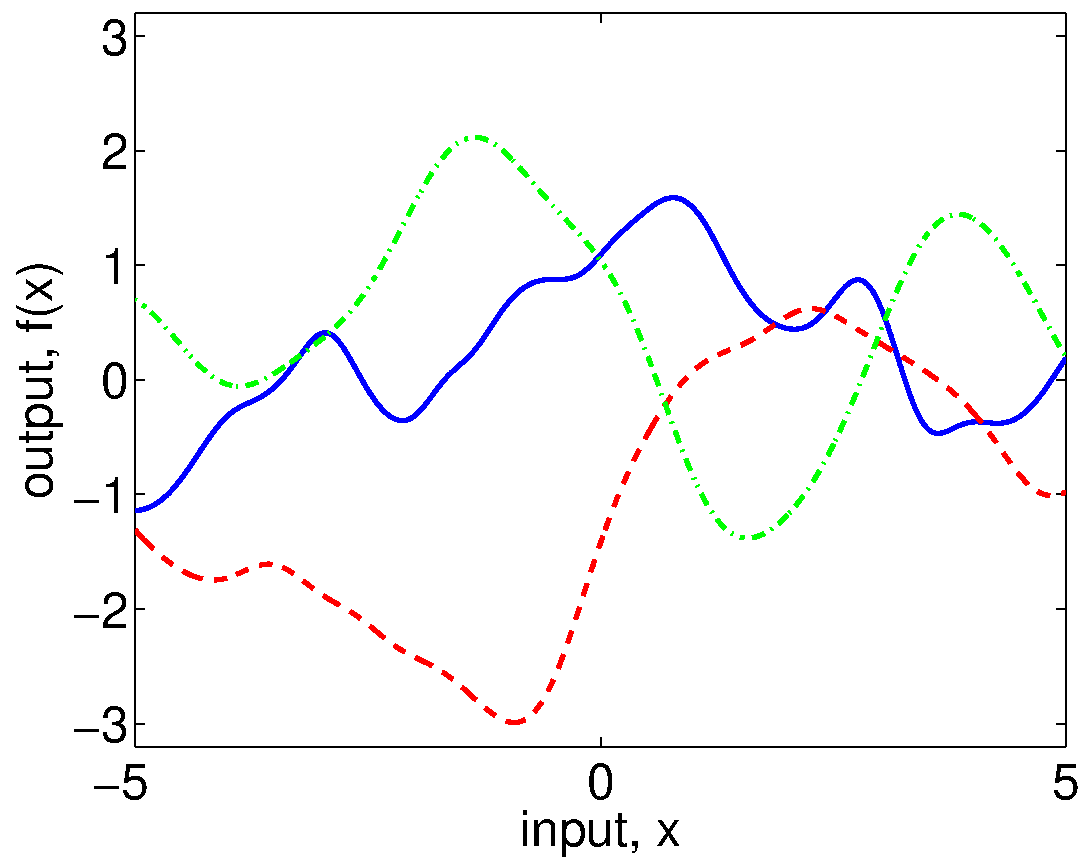
\includegraphics[width=0.45\textwidth]{rq2}
\end{tabular}
\end{center}

The limit $\alpha\rightarrow\infty$ of the RQ covariance function is the SE.

\end{frame}

\begin{frame}
\frametitle{Matérn covariance functions}

Stationary covariance functions can be based on the Matérn form:
\[
k({\bf x},{\bf x}')=\frac{1}{\Gamma(\nu)2^{\nu-1}}\Big[
\frac{\sqrt{2\nu}}{\ell}|{\bf x}-{\bf x}'|\Big]^\nu K_\nu
\Big(\frac{\sqrt{2\nu}}{\ell}|{\bf x}-{\bf x}'|\Big),
\]
where $K_\nu$ is the modified Bessel function of second kind of order $\nu$,
and $\ell$ is the characteristic length scale.

Sample functions from Matérn forms are $\lfloor \nu-1\rfloor$ times
differentiable. Thus, the hyperparameter $\nu$ can control the degree of
smoothness

Special cases:
\begin{itemize}
\item $k_{\nu=1/2}(r)=\exp(-\frac{r}{\ell})$: Laplacian covariance function,
Brownian motion (Ornstein-Uhlenbeck)
\item $k_{\nu=3/2}(r)=\big(1+\frac{\sqrt{3}r}{\ell}\big)
\exp\big(\!-\frac{\sqrt{3}r}{\ell}\big)$ (once differentiable)
\item $k_{\nu=5/2}(r)=\big(1+\frac{\sqrt{5}r}{\ell}+\frac{5r^2}{3\ell^2}\big)
\exp\big(\!-\frac{\sqrt{5}r}{\ell}\big)$ (twice differentiable)
\item $k_{\nu\rightarrow\infty}=\exp(-\frac{r^2}{2\ell^2})$: smooth
(infinitely differentiable)
\end{itemize}
\end{frame}

\begin{frame}
\frametitle{Matérn covariance functions II}

Univariate Matérn covariance function with unit characteristic length scale
and unit variance:

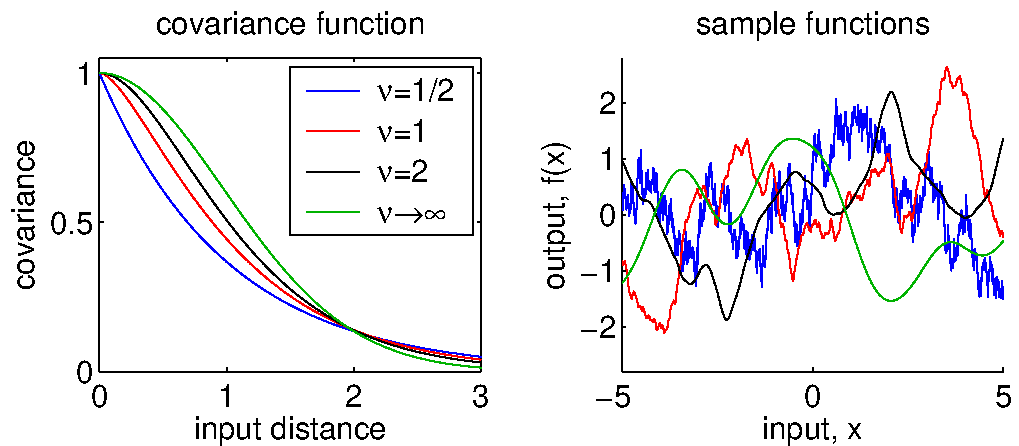
\includegraphics[width=\textwidth]{matern}
\end{frame}


\begin{frame}
\frametitle{Periodic, smooth functions}
To create a distribution over periodic functions of $x$, we can first map the
inputs to $u=(\sin(x),\cos(x))^\top$, and then measure distances in the $u$
space. Combined with the SE covariance function, which characteristic length
scale $\ell$, we get:
\[
k_{\rm periodic}(x,x')\;=\;\exp(-2\sin^2(\pi(x-x'))/\ell^2)
\]
\begin{center}
\begin{tabular}{cc}
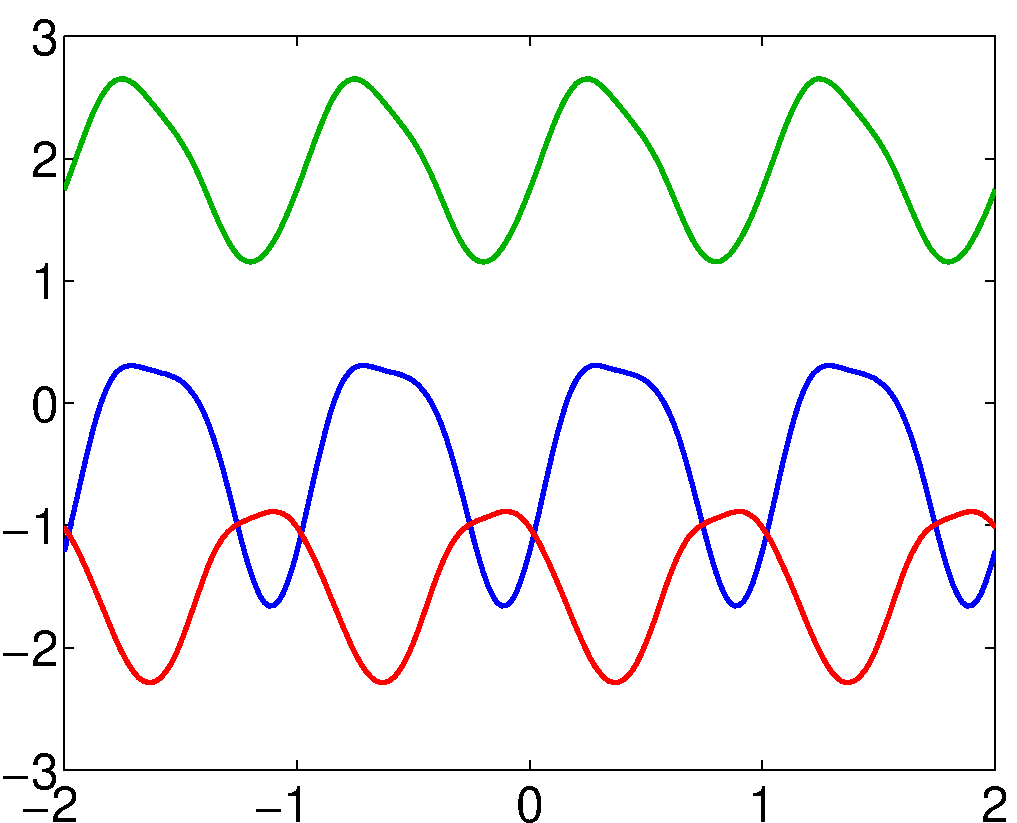
\includegraphics[width=0.45\textwidth]{per00} &
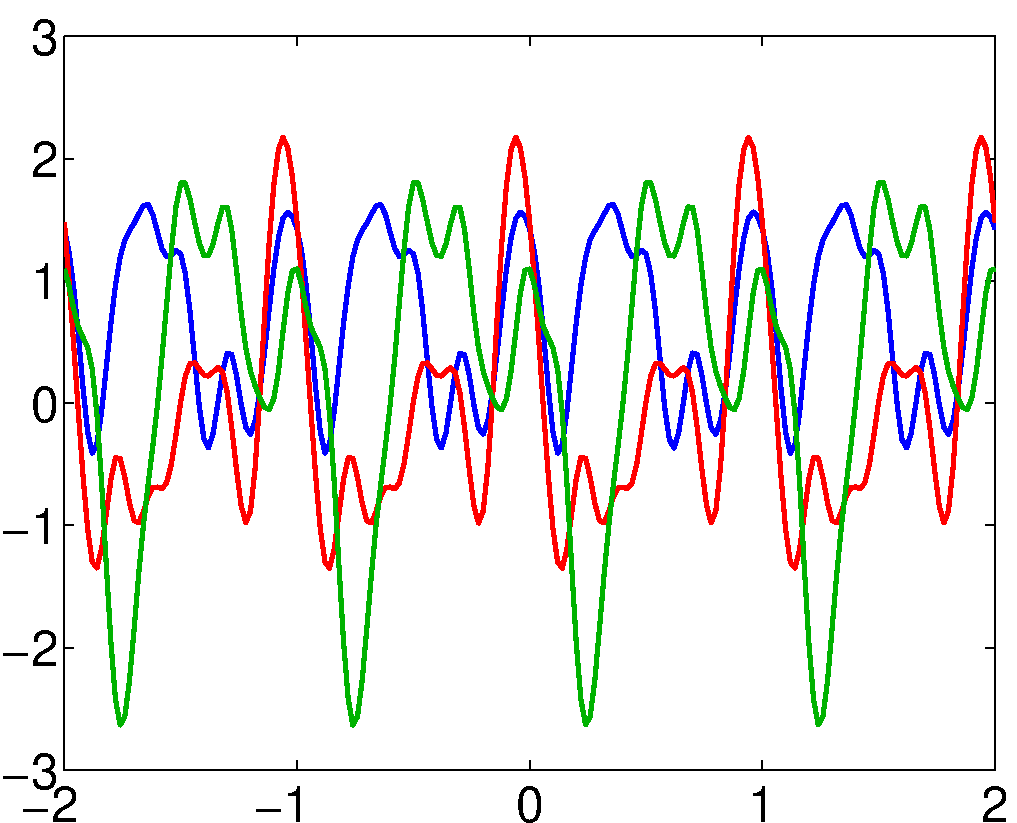
\includegraphics[width=0.45\textwidth]{per01}
\end{tabular}
\end{center}
Three functions drawn at random; left $\ell>1$, and right $\ell<1$.
\end{frame}


\begin{frame}
\frametitle{Spline models}

One dimensional minimization problem: find the function $f(x)$ which minimizes:
\[
\sum_{i=1}^c(f(x^{(i)})-y^{(i)})^2+\lambda\int_0^1(f''(x))^2dx,
\]
where $0<x^{(i)}<x^{(i+1)}<1,\;\forall i=1,\dots, n-1$, has as solution the 
\Blue{Natural Smoothing Cubic Spline}: first order polynomials when
$x\in[0;x^{(1)}]$
and when $x\in[x^{(n)};1]$ and a cubic polynomical in each
$x\in[x^{(i)};x^{(i+1)}],\;\forall i=1,\ldots,n-1$, joined to have
continuous second derivatives at the knots.

The identical function is also the mean of a Gaussian process:
Consider the class a functions given by:
\[
f(x) = \alpha + \beta x + \lim_{n\rightarrow\infty}\frac{1}{\sqrt{n}}
\sum_{i=0}^{n-1}\gamma_i(x-\frac{i}{n})_+,
\qquad\text{where\ }(x)_+=\begin{cases}x&\text{\ if\ }x>0\\ 0&\text{\ otherwise}
\end{cases}
\]
with Gaussian priors:
\[
\alpha\sim{\cal N}(0,\xi),\quad
\beta\sim{\cal N}(0,\xi),\quad
\gamma_i\sim{\cal N}(0,\Gamma),\;\forall i=0,\ldots,n-1.
\]
\end{frame}

\begin{frame}
The covariance function becomes:
\[
\begin{split}
k(x,x')\;=&\;\xi+xx'\xi +
\Gamma\lim_{n\rightarrow\infty}\frac{1}{n}\sum_{i=0}^{n-1}
(x-\frac{i}{n})_+\;(x'-\frac{i}{n})_+\\
=&\;\xi+xx'\xi + \Gamma\int_0^1(x-u)_+\;(x'-u)_+du\\
=&\;\xi+xx'\xi +
\Gamma\big(\frac{1}{2}|x-x'|\min(x,x')^2+\frac{1}{3}\min(x,x')^3\big).
\end{split}
\]
In the limit $\xi\rightarrow\infty$ and $\lambda=\sigma^2_n/\Gamma$
the posterior mean becomes the natrual cubic spline.

We can thus find the hyperparameters $\sigma^2$ and $\Gamma$ (and
thereby $\lambda$) by maximising the marginal likelihood in the usual
way.

Defining $h(x)=(1,x)^\top$ the posterior predictions with mean and variance:
\[
\begin{split}
\tilde\mu(X_*)\;&=\;H(X_*)^\top\beta+K(X,X_*)[K(X,X)+\sigma_n^2I]^{-1}({\bf y}-H(X)^\top\beta)\\
\tilde\Sigma(x_*)\;&=\;\Sigma(X_*)+R(X,X_*)^\top A(X)^{-1}R(X,X_*)\\
\beta\;&=\;A(X)^{-1}H(X)[K+\sigma_n^2I]^{-1}{\bf y},\quad
A(X) = H(X)[K(X,X)+\sigma_n^2I]^{-1}H(X)^\top\\
R(X,X_*)\;&=\;H(X_*)-H(X)[K+\sigma^2_nI]^{-1}K(X,X_*)
\end{split}
\]
\end{frame}


\begin{frame}
\frametitle{Cubic Splines, Example}

Although this is not the fastest way to compute splines, it offers
a principled way of finding hyperparameters, and uncertainties on predictions.

Note also, that although the \Blue{posterior mean} is smooth
(piecewise cubic), posterior sample functions are not.

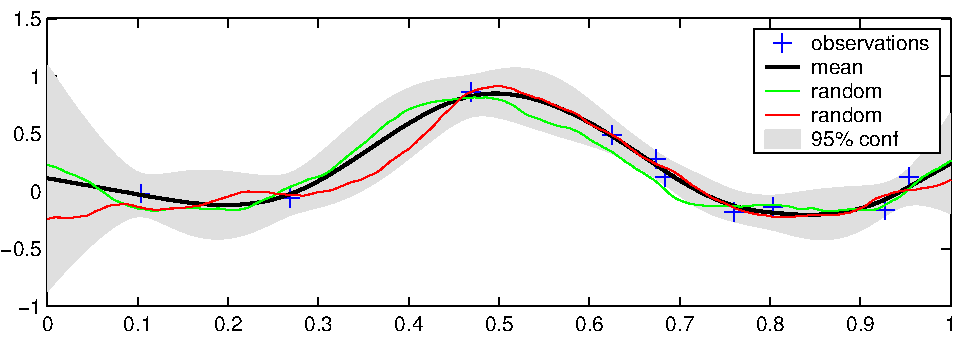
\includegraphics[width=\textwidth]{gpsplines}
\end{frame}


\begin{frame}
\frametitle{Feed Forward Neural Networks}
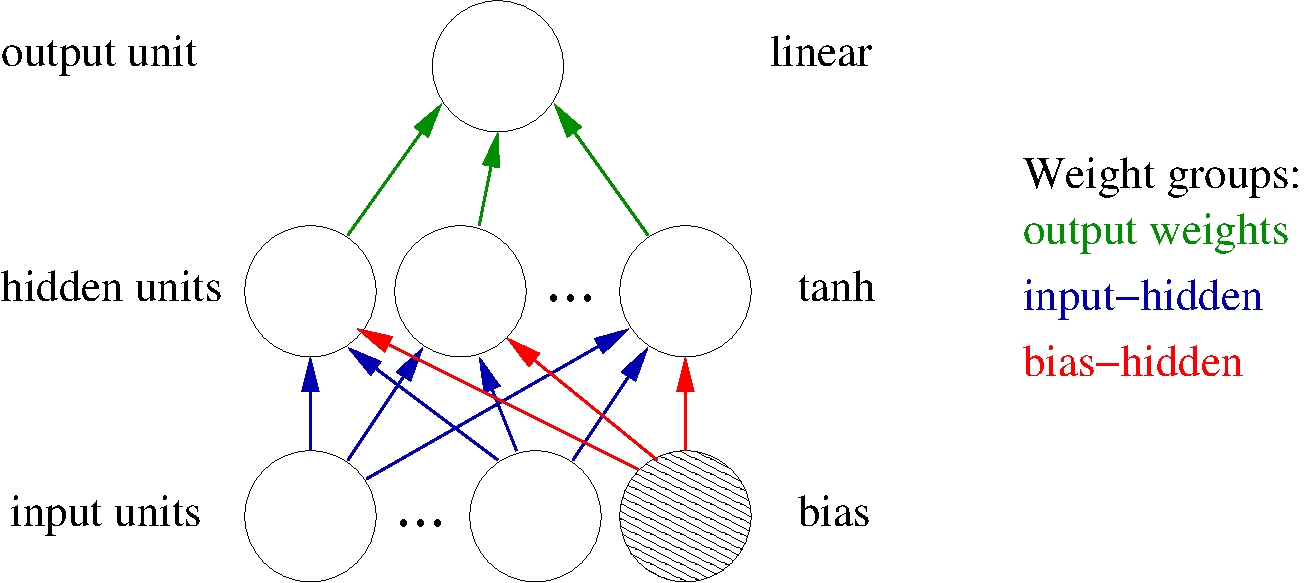
\includegraphics[width=\textwidth]{network}

A feed forward neural network implements the function:
\[
f(x)\;=\;\sum_{i=1}^H v_i\tanh(\sum_j u_{ij}x_j+b_j)
\]
\end{frame}

\begin{frame}
\frametitle{Limits of Large Neural Networks}
Sample random neural network weights from a appropriately scaled Gaussian prior.

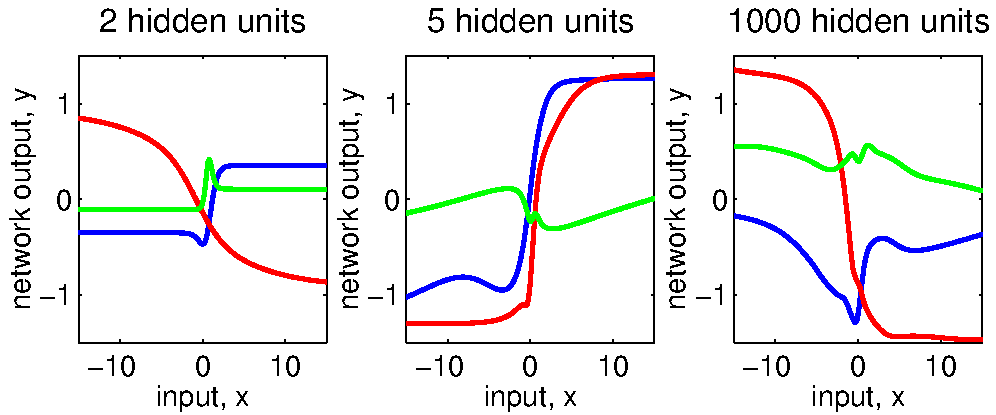
\includegraphics[width=\textwidth]{networkprior}

Note: The prior on the neural network weights \emph{induces} a prior over
functions.
\end{frame}


\begin{frame}
\begin{center}
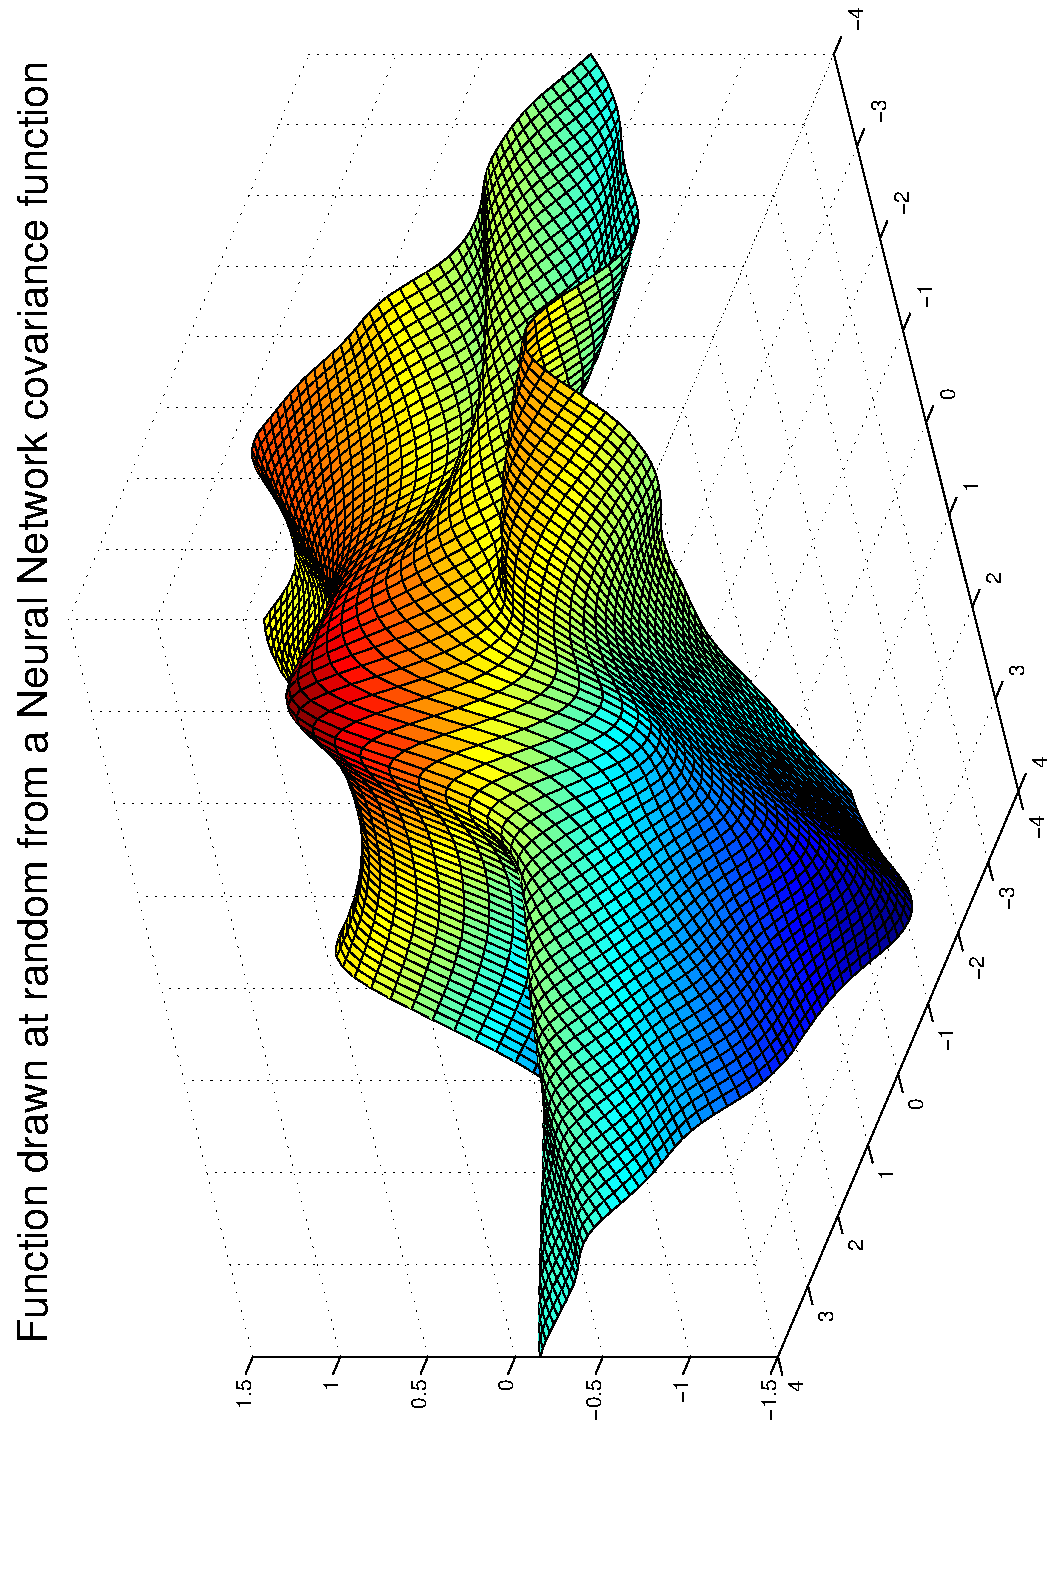
\includegraphics[height=0.85\textwidth,angle=-90]{gpprior2}
\end{center}
\[
k(x,x')\;=\;\frac{2}{\pi}\arcsin\big(\frac{2x^\top\Sigma x'}{\sqrt{(1+x^\top
\Sigma x)(1+2x'^\top\Sigma x')}}\big).
\]
\end{frame}


\begin{frame}
\frametitle{Composite covariance functions}

We've seen many examples of covariance functions.\\[1ex]

Covariance functions have to be \Blue{possitive definite}.\\[1ex]

One way of building covariance functions is by composing simpler ones
in various ways
\begin{itemize}
\item sums of covariance functions $k(x,x') = k_1(x,x') + k_2(x,x')$
\item products $k(x,x') = k_1(x,x') \times k_2(x,x')$
\item other combinations: $g(x)k(x,x')g(x')$
\item etc.
\end{itemize}
The gpml toolbox supports such constructions.
\end{frame}
\end{document}